\let\mymarginpar\marginpar

\documentclass[11pt,twoside]{article}

%\long\def\authornote#1{%
%        \leavevmode\unskip\raisebox{-3.5pt}{\rlap{$\scriptstyle\diamond$}}%
%        \marginpar{\raggedright\hbadness=10000
%        \def\baselinestretch{0.8}\tiny
%        \it #1\par}}
%\newcommand{\ville}[1]{\authornote{NOTE TO SELF: #1}}

\marginparwidth=1cm
\marginparsep=5pt
\newcommand\ville[1]{%
    \mymarginpar{\raggedright\hbadness=10000\tiny\it #1\par}}


\usepackage{amsmath} 
\usepackage{times}
\usepackage{amsmath,amsthm,amssymb}
\usepackage{fancyhdr}
\usepackage{moreverb}
\usepackage{graphicx}
\usepackage{amssymb}
\usepackage{url}
\usepackage{multirow} 
\usepackage[boxed, section]{algorithm}
%\usepackage{algorithm}
\usepackage{algorithmic}
\usepackage{cite}
\usepackage{multirow} 
\usepackage{rotating}
\usepackage{geometry}
\usepackage{fix-cm}
\usepackage{subfigure}
\usepackage{natbib}


\renewcommand{\baselinestretch}{1.2}
\setlength{\topmargin}{-0.3in}
\setlength{\textwidth}{6in}
\setlength{\textheight}{8.5in}
\setlength{\oddsidemargin}{0.25in}
\setlength{\evensidemargin}{0.25in}
\raggedbottom




\allowdisplaybreaks

% Math Macros.  It would be better to use the AMS LaTeX package,
% including the Bbb fonts, but I'm showing how to get by with the most
% primitive version of LaTeX.  I follow the naming convention to begin
% user-defined macro and variable names with the prefix "my" to make it
% easier to distiguish user-defined macros from LaTeX commands.
%
\newcommand{\myN}{\hbox{N\hspace*{-.9em}I\hspace*{.4em}}}
\newcommand{\myZ}{\hbox{Z}^+}
\newcommand{\myR}{\hbox{R}}
\renewcommand{\P}{\mathbb{P}}
\newcommand{\E}{\mathbb{E}}
\newtheorem{defi}{Definition}
\newtheorem{theorem}{Theorem}[section]
\newtheorem{lemma}[theorem]{Lemma}

\newcommand{\myfunction}[3]
{${#1} : {#2} \rightarrow {#3}$ }

\newcommand{\myzrfunction}[1]
{\myfunction{#1}{{\myZ}}{{\myR}}}


\newcommand{\mysection}[1]
{\noindent {\bf {#1}}}

%%%%%% Begin document with header and title %%%%%%%%%

\begin{document}

\title{Information Theoretic Alternative to Signal Generation with an Application to Principled Probability Extremization}
%\title{A Novel Framework for Analyzing Subjective Response Data}
\author{
Ville A. Satop\"a\"a, Robin Pemantle, and Lyle H. Ungar\\
\\
 \small Department of Statistics\\
 \small The Wharton School of the University of Pennsylvania\\
 \small Philadelphia, PA 19104- 6340, USA\\ [-0.25in]} \date{}
\maketitle

\pagestyle{myheadings}
\markboth{Information Theoretic Signal Generation}{Satop\"a\"a et al.}
\thispagestyle{empty}

\begin{abstract}
Typically randomness in scientific measurements is assumed to arise from unmeasured or uncontrolled factors. This paper presents an information theoretic framework that introduces an alternative source of randomness. This framework, which is particularly appropriate for subjective response data, is illustrated on probability aggregation. The probabilities are given by a group of experts who forecast whether an event will occur or not. Our aggregator uses the distribution of information among the experts and depends on easily interpretable parameters. Even though shifting the average probability forecasts closer to its nearest extreme, known as \textit{extremizing}, is known to yield improved forecast performance, it is much less understood when and how much the average forecast should be extremized. By assuming a simplified information structure in our model, the amount of extremizing is studied closely under different values of  the parameters. This leads to novel observations and a more principled understanding of extremization.
\end{abstract}

%data generative process. 


\section{Introduction}
Experts are often required to form estimates under incomplete information. These estimates can be made in several ways. Currently the two main approaches classify the estimate either as \textit{generated} or \textit{interpreted} (\cite{hong2009interpreted}). The estimate is called generated if the expert is assumed to sample the estimate from a given probability distribution. For instance, estimating the length of an object with a ruler can be assumed to be equivalent to drawing a value from a symmetric distribution, such as the Gaussian distribution, centered at the true length. An estimate is said to be interpreted if the expert first filters reality into set of categories and then makes an estimate by applying active cognitive effort to these categories. For instance, the score given by an Olympic judge on a figure skating performance can be considered interpreted. The judge has his personal set of criteria (categories) that ultimately decides the score. 

The interpreted framework is clearly a more realistic model for subjective response data. Given that such data is very common in real-world applications, such as product reviews, online auctions, and voting, this framework is a great advance in understanding the gap between experimental and real-world results. Unfortunately, it is too general to be useful in developing novel methodology. First,  interpretations differ between individuals and arise from a complex cognitive process that can be very difficult to estimate. Second, it is unclear how to construct the model to incorporate all the information that is used in making these interpretations.


The first contribution of this paper is to introduce a novel framework for signal generation. This framework, that is called \textit{information theoretic}, is based on the distribution of information among the experts. Each expert gives an estimate solely based on his personal information set. The information set includes any internal factors, such as personal preferences and interpretation criteria, and external factors, such as knowledge of the target event, that affect the estimation process. Therefore two overlapping information sets are assumed to produce positively correlated estimates. This framework, which is a good compromise between the psychological and analytical models, is much more amenable for development of future methodology. 

The second contribution of this paper is to illustrate the information theoretic framework  on probability aggregation. Combining multiple probability forecasts is an important problem with many applications including medical diagnosis (\citet{wilson1998prediction, pepe2003statistical}), political and socio-economic foresight (\citet{tetlock2005expert}), and meteorology (\citet{sanders1963subjective, vislocky1995improved, baars2005performance}). There is strong empirical evidence that bringing together the strengths of different experts by combining their probability forecasts into a single consensus, known as the \textit{crowd belief},  improves predictive performance. Recent developments suggest that shifting the average probability closer to its nearest extreme (0.0 or 1.0), known as \textit{extremizing}, yields even further improvements in forecasting performance. For instance, \citet{satopaa} uses a linear regression model in the logit-space to derive an extremizing aggregator that performs well on real-world data. \citet{Ranjan08} propose transforming the average probability with the CDF of a beta distribution. If both the shape and scale of this beta distribution are equal and constrained to be at least 1.0,  the aggregator extremizes and has some attractive theoretical properties (\cite{Wallsten2001}).  \citet{Baron} provide  two intuitive justifications for extremizing.

%To give an intuitive justification for extremization,  consider a binary event whose outcome is still uncertain.  For the sake of illustration, assume that 0.9 is the most informed probability forecast that could be given based on all the available information. Before having any knowledge of the event, a rational forecaster aiming to minimize a reasonable loss function, such as the Brier score, has no reason to give anything but 0.5 as his probability forecast. In the Bayesian terminology, this estimate can be viewed as his prior belief. As he acquires more information, he updates his prior belief accordingly.  This updated belief, which can be viewed as his posterior belief, is a compromise between his prior belief and the information acquired. Because he does not have all the available information, his estimate is conservative and necessarily too close to 0.5. If most forecasters fall somewhere on this spectrum between ignorance and full information, their average forecast tends to fall strictly between 0.5 and 0.9. It this difference between the ``true probability" and the average forecast that extremization aims to close. 

The current extremizing aggregators have several shortcomings. First, often the underlying assumptions are overly simplistic or too detached from the psychology literature to provide the researcher any insight beyond the aggregate probability. For instance, it is still not well-understood when and how much should the average probability be extremized. Therefore it is necessary to learn the amount of extremizing from a separate training dataset. Second, the aggregators often arise from regression analysis that assumes the measurements to deviate from the truth by a random amount. Given that this random deviation is typically assumed to have a mean of zero, the true parameter values are estimated by a form of averaging. It is unlikely that this framework, under which estimation is performed via simple averaging, is appropriate for probability aggregation because extremizing the average probability forecast is known to improve its forecasting performance.

The first contribution of this paper is to introduce an information theoretic framework that offers an alternative interpretation for the source of randomness in scientific measurements. This framework can be especially useful for analyzing subjective response data. The second contribution of this paper is to illustrate our framework by deriving an information theoretic model for probability aggregation. The aggregator is based on the distribution of information among experts who are forecasting the outcome of a binary event.  Under this model the average forecast is always extremized, and the amount of extremization is available in a closed-form. Given that this form depends on three parameters,  the number of experts, the amount of information known by an expert, and the amount of information shared by two experts, it allows us to investigate when and how much extremization should be performed. 

This paper is structured as follows. The first section introduces our information theoretic framework and  compares it with the classical data generative process from regression analysis. The framework is then illustrated on probability aggregation. The aggregator provides an general closed-form expression for the amount of extremization. This form is analyzed in full generality and under a compound symmetric information structure. This simplified structure allows us to discuss and understand extremization in terms of a few intuitive parameters. The paper concludes with a discussion of  model limitations and future directions. 



\section{Information Theoretic Framework}
This section illustrates some of the similarities and differences between our information theoretic framework and the classical data generative process from regression analysis. This comparison is by no means comprehensive as regression analysis encompasses a very vast literature in statistics. The main difference is in the way the two frameworks incorporate randomness.

\begin{figure}[htbp]
   \centering
   \includegraphics[width = 0.6\textwidth]{regression} % requires the graphicx package
   \caption{Comparison of the physical and information theoretic frameworks.}
   \label{framework}
\end{figure}


To guide our comparison, Figure \ref{framework} illustrates both setups with the regression framework on the left and the information theoretic framework on the right. The two large circles represent the set of relevant factors, or simply the universe. This is the same under both frameworks. Consider first the regression framework on the left side. From the experimenter's point of view, the universe is divided into controlled (C) and uncontrolled factors (U) that affect his measurement (Y). The uncontrolled factors are assumed to have a random effect, typically with mean of zero, on the measurement. Therefore any repeated measurement under the same set of controlled factors leads to a slightly different answer.  


The right side of Figure \ref{framework} depicts our information theoretic framework. Under this framework the data are generated by first picking a random subset of factors from the universe. This subset is then assumed to form its own sub-universe, where all factors are controlled. Repeating the measurement in this sub-universe always leads to the same answer (Z). Therefore, while in the regression framework any differences between two measurements is assumed to arise from the uncontrolled factors, these differences in the information theoretic framework arise due to different sets of sub-universes. In both cases the differences are random. 

The need for our information theoretic framework is becomes clear by considering subjective responses. For instance, the response variable in the study may be the subject's personal belief about the closing price of a particular capital stock. The person in this case forms the sub-universe depicted by the small circle in Figure \ref{framework}. He holds some subset of  the information that make up the universe. He uses his information efficiently to produce an answer that is his \textit{personal truth}. There is no noise in his answer. Therefore, if he is asked the same question immediately after, he gives the same response. If, on the other hand, he is asked the same question a day later, he may give a different answer because his information set may have changed by then. 

It is unclear how subjective responses can arise from the regression framework because under this setup exact measurements are not possible. Furthermore, repeated measurements cannot be identical. Instead they differ by a random amount that is often assumed to have a mean of zero. Therefore averaging can help to smooth the data and reveal a better picture of the underlying truth. But as has been shown in previous literature, mere averaging does not lead to optimal probability aggregation. The average must be extremized. Therefore the regression context does not appear suitable for analyzing probability forecasts. The next section introduces a information theoretic model for analyzing probability forecasts. 


%In regression analysis the observations are assumed to deviate from the truth due to randomness that arises from the combined influence of many unobservable conditions. Averaging can help to smooth the data and reveal a better picture of the underlying truth. As have been shown in previous literature, mere averaging does not lead to optimal probability aggregation. The average must be extremized. Therefore the regression context does not appear suitable for analyzing probability forecasts. 
%
%Our framework does not assume unobservable conditions. Instead, each observation represents the truth under the given set of conditions. This means that if another measurement was to be performed under the same conditions, the resulting observation would be the same as before. Therefore any differences between observations are caused by variations in the underlying conditions. 
%
% the randomness arises from different information sets. 
%


%
%
%
%Consider the model
%\begin{align}
%X_S &= \sum_{i=1}^\infty \beta_i X_i, \label{regression}
%\end{align}
%where the full process $X_s$ is a weighted sum of countably many ``facts" denoted with $X_i$. Assume now that the expert holds only some subset of these ``facts." Call this set $\textit{I}_{1}$ and let $\mathcal{I}_0 = \mathbb{N} / \mathcal{I}_1$ be the set unknown to the expert. Equation (\ref{regression}) then breaks down to known and unknown terms
%\begin{align*}
%X_S &= \sum_{i \in \mathcal{I}_1} \beta_i X_i + \sum_{i \in \mathcal{I}_0} \beta_i X_i,
%\end{align*}
% Denoting the experts probit forecast with $Y$, the unknown component with $\epsilon$, and reordering some of them terms we have that 
%\begin{align*}
%Y &= X_S + \epsilon
%\end{align*}
%The term $\epsilon$ is considered noise and typically assumed to have a mean of zero. Under this model averaging multiple probit forecasts $\{ Y_j \}_{j=1}^N$, gives an unbiased estimator of $X_S$. As have been shown in literature, mere averaging does not lead to optimal probability aggregation. The average must be extremized. Therefore the regression context does not appear suitable for analyzing probability forecasts. 
%
%In the next section we show that our framework leads to very intuitive extremization. The average probit forecast is always extremized. Another difference is in the way the noise term is treated. In our model any deviation from $X_S$ is caused by a constant -- not random -- $\epsilon$. Therefore in our framework any two experts holding the same set of ``facts" would give identical forecasts. This means that the decision-making is solely based on the information set that the expert has. In the regression context, on other hand, the two experts would give slightly different probit forecasts because the realization of the random $\epsilon$ is different for them. 
%
%WHERE DOES RANDOMNESS ARISE IN EACH CASE. 

\section{Model for Probability Forecasts}
\label{Model}
Consider a probability space $(\Omega, \mathcal{F}, \P)$ and an event $A \in \mathcal{F}$ to be forecasted. Expert $j$ knows information $\mathcal{F}_j \subseteq \mathcal{F}$ and forecasts $p_j = \P(A | \mathcal{F}_j)$. The best in-principle forecast given the knowledge of the $N$ forecasters is $P(A | \mathcal{F}')$, where $\mathcal{F}' = \mathcal{F}_1 \cup \mathcal{F}_2 \cup .. \cup \mathcal{F}_N$. As in this work we do not allow the experts to exchange information with each other, the best aggregate probability is given by $\P(A | p_1, p_2, \dots, p_N)$.

For illustrative purposes, we first assume only two experts and then generalize the model to $N$ experts. Under our model the event $A$ is determined by a pool of white noise. Experts 1 and 2 see respective $\delta_1$ and $\delta_2$ portions of the noise. These portions form their information sets. The overlap in their information sets is a fixed share $\rho$ of what is seen by either expert. This can be made more precise by letting  $(\Omega, \mathcal{F}, \P)$ be a probability space on which we define a white noise process indexed by the unit interval $S$. A white noise process is a Gaussian process $\{ X_B \}$ indexed by Borel measurable subsets $B$. We endow the unit interval with the uniform measure, $\mu$. This gives the white noise process a covariance structure of $Cov(X_B, X_{B'}) = \mu(B \cap B') = |B \cap B'|$, i.e. the length of the intersection. The target event is defined as $A = \{ X_{S} > 0\}$. Let $I_1, I_2 \subseteq S$ be the information sets observed by experts 1 and 2, respectively. Thus,
\begin{align*}
\mu(I_1) = |I_1| &= \delta_1\\
\mu(I_2) = |I_2| &= \delta_2\\
\mu(I_1 \cap I_2) =  |I_1 \cap I_2| &= \rho
\end{align*}
Call $X_{I_j}$ the probit forecast of the $j$th expert.  If $\Phi$ denotes the standard normal CDF, then
\begin{align*}
p_j &= \P(A | \mathcal{F}_{I_j}) = \Phi(X_{I_j})
\end{align*}
for $j = 1, 2$, and the aggregator is given by $\P(X_{S} > 0 | p_1, p_2)$.

\begin{figure}[htbp]
%   \hspace{-2em}
   \includegraphics[width = \textwidth]{N=2} % requires the graphicx package
   \caption{Illustration of the model with two experts.}
   \label{diagram2}
\end{figure}

Figure \ref{diagram2} illustrates the model with $N=2$. The Gaussian process has been partitioned into four parts based on the information sets $I_1$ and $I_2$:
\begin{align*}
 U &= X_{I_1 / I_2}\\
M &= X_{I_1 \cap I_2}\\
V &= X_{I_2 / I_1}\\
W &= X_{(I_1 \cup I_2)^c}
\end{align*}
Then $X_{I_1} = U + M$, $X_{I_2} = M + V$, and $X_S = U+M+V+W$, where $U, V, M, W$ are independent Gaussians with respective variances $\delta_1-\rho$, $\delta_2-\rho$, $\rho$, $1+\rho-\delta_2 - \delta_3$. This gives $(X_{S}, X_{I_1}, X_{I_2})$ a multivariate normal distribution. More specifically, we have 
\begin{align}
\left(\begin{matrix} X_S \\ X_{I_1}\\ X_{I_2} \end{matrix}\right) &\sim \mathcal{N}\left(
 \boldsymbol{0},  \left(\begin{matrix} 
1 & \delta_1 & \delta_2\\
\delta_1 & \delta_1 &\rho\\
\delta_2 & \rho & \delta_2
 \end{matrix}\right)\right) \label{twoExperts}
\end{align}

\begin{figure}[htbp]
   \includegraphics[width = \textwidth]{N=N} % requires the graphicx package
   \caption{Illustration of the model with $N$ experts.}
   \label{diagramN}
\end{figure}



Consider now $N$ experts. Let $|I_j| = \delta_j$ be the amount of information known by the $j$th expert, and $|I_i \cap I_j| = \rho_{ij}$ be the information overlap between the $i$th and $j$th experts. Then expression (\ref{twoExperts}) generalizes to the vector $(X_{S}, X_{I_1}, X_{I_2}, \dots, X_{I_N})$. This gives us
\begin{align*}
\left(\begin{matrix} X_S \\ X_{I_1}\\ \vdots \\ X_{I_N} \end{matrix}\right) &\sim \mathcal{N}\left( \left(\begin{matrix} 
\mu_1 \\ \boldsymbol{\mu}_2
 \end{matrix}\right) =
 \boldsymbol{0}, \left(\begin{matrix} 
\Sigma_{11} & \Sigma_{12}\\
\Sigma_{21} & \Sigma_{22}\\
 \end{matrix}\right) 
 =
 \left(\begin{array}{c | c c cc }
1 & \delta_1 & \delta_2 & \dots & \delta_N  \\ \hline
\delta_1 & \delta_1 &\rho_{1,2} & \dots & \rho_{1,N}   \\ 
\delta_2 & \rho_{2,1} & \delta_2 & \dots & \rho_{2,N}  \\ 
\vdots & \vdots & \vdots & \ddots & \vdots  \\ 
\delta_N & \rho_{N,1} & \rho_{N,2} & \dots & \delta_N\\ 
 \end{array}\right)\right)
\end{align*}
This is illustrated in Figure \ref{diagramN}. It is important to notice that the $I_j$ does not have to be contiguous segment of the unit interval. The sub-matrix $\Sigma_{22}$ fully describes the information structure among the experts.  This matrix has some technical conditions such as symmetry and non-singularity. In addition, $\Sigma_{22}$ must describe a coherent information structure. The matrix $\Sigma_{22}$ is coherent if and only if its information can be transformed into a diagram such as the one depicted by Figure \ref{diagramN}.



%Thus $\bar{X}$ is extremized when
%\begin{align*}
% \frac{N \boldsymbol{1}_{N}' \Sigma_{22}^{-1} \boldsymbol{X}}{\boldsymbol{1}_{N}'  \boldsymbol{X}  \sqrt{N - \boldsymbol{1}_{N}' \Sigma_{22}^{-1} \boldsymbol{1}_{N}}}   &>& 1\\
% \frac{\boldsymbol{1}_{N}' \Sigma_{22}^{-1} \boldsymbol{X}}{\boldsymbol{1}_{N}'  \boldsymbol{X}  }   &>& \sqrt{ \frac{1}{N} - \frac{\boldsymbol{1}_{N}' \Sigma_{22}^{-1} \boldsymbol{1}_{N}}{N^2}},
%\end{align*}
%where the LHS side a weighed average of the elements of $\Sigma_{22}^{-1}$. This becomes clear after noticing that $\boldsymbol{X} / \boldsymbol{1}_{N}'  \boldsymbol{X}$ is a vector whose elements sum to 1. These give the weights for each respective column of $\Sigma_{22}^{-1}$. Hence the larger a given $X_j$ is the more influence it has in his weighted sum. The second term on RHS is the equally weighed average of $\Sigma_{22}^{-1}$. Notice that LHS increases as a function of $\Sigma_{22}^{-1}$ while RHS decreases. In addition, if $\boldsymbol{1}_{N}' \Sigma_{22}^{-1}  \boldsymbol{1}_{N} > \approx 1.1$ and fixed, then RHS decreases as $N$ increases. This largely revolves around understanding the interpretation of the precision matrix. 
%
%\begin{align*}
% \frac{( \boldsymbol{1}_{N}' \Sigma_{22}^{-1} \boldsymbol{X} )( \boldsymbol{X}'  \Sigma_{22}^{-1}\boldsymbol{1}_{N} )}{(\boldsymbol{1}_{N}'  \boldsymbol{X} )(  \boldsymbol{X}'  \boldsymbol{1}_{N})}   &>& \frac{1}{N} - \frac{\boldsymbol{1}_{N}' \Sigma_{22}^{-1} \boldsymbol{1}_{N}}{N^2}\\
%\end{align*}


\section{Extremization}
Let $\boldsymbol{X}$ be a column vector of length $N$ such that $X_j = X_{I_j}$. If $\Sigma_{22}$ is a coherent overlap structure such that $\Sigma_{22}^{-1}$ exists, then $X_{S} | \boldsymbol{X} \sim \mathcal{N}(\bar{\mu}, \bar{\Sigma})$, where
\begin{align}
\bar{\mu} &= \mu_1 + \Sigma_{12} \Sigma_{22}^{-1} (\boldsymbol{X} - \boldsymbol{\mu}_2) =  \Sigma_{12} \Sigma_{22}^{-1} \boldsymbol{X} \label{condMu}
\end{align}
and
\begin{align}
 \bar{\Sigma}&= \Sigma_{11} - \Sigma_{12} \Sigma_{22}^{-1} \Sigma_{21} =1 - \Sigma_{12} \Sigma_{22}^{-1} \Sigma_{21}  \label{condSigma}
\end{align}
See Result 5.2.10 on p. 156 in \cite{ravishanker2001first} for the formulas of a conditional multivariate normal distribution. The aggregator then becomes 
\begin{align*}
\P\left(A  \bigg| \boldsymbol{X}\right)  = \P\left(X_{S} > 0 \bigg| \boldsymbol{X}\right) &= \Phi\left( \frac{\Sigma_{12} \Sigma_{22}^{-1} \boldsymbol{X}}{\sqrt{1 - \Sigma_{12} \Sigma_{22}^{-1} \Sigma_{21}}}\right)
%&= \Phi\left( \frac{\boldsymbol{1}_{N}'  \Sigma_{22}^{-1} \Phi^{-1}(\boldsymbol{p})}{\sqrt{1 - \boldsymbol{1}_{N}' \Sigma_{22}^{-1} \boldsymbol{1}_{N}}}\right)
\end{align*}
Let $\alpha$ represents the amount of extremization that is performed for the average probit forecast. If $\bar{X}$ denotes the sample average, then
\begin{align}
\alpha \bar{X}&=  \frac{\Sigma_{12} \Sigma_{22}^{-1} \boldsymbol{X}}{\sqrt{1 - \Sigma_{12} \Sigma_{22}^{-1} \Sigma_{21}}}  &\Leftrightarrow&& \alpha  = \frac{N \Sigma_{12} \Sigma_{22}^{-1} \boldsymbol{X}}{\left(\boldsymbol{1}_N' \boldsymbol{X} \right) \sqrt{1 - \Sigma_{12} \Sigma_{22}^{-1} \Sigma_{21}}} \label{alpha}
\end{align}
Even though this expression assumes no structure on $\Sigma_{22}$ and depends on $N +\frac{N(N-1)}{2}$ unknown parameters, it can be used to gain insight on the behavior of the extremizing constant, $\alpha$. One useful development is to determine the amount of information in $\boldsymbol{X}$. 

\begin{lemma}
\label{infoLemma}
If $\delta_0$ denotes the information in $\boldsymbol{X}$, then 
\begin{align*}
%\frac{N \Sigma_{12} \Sigma_{22}^{-1} \boldsymbol{X}}{\left(\boldsymbol{1}_N' \boldsymbol{X} \right) \sqrt{1 - \Sigma_{12} \Sigma_{22}^{-1} \Sigma_{21}}} &= \alpha\\
%\frac{\Sigma_{12} \Sigma_{22}^{-1} }{\sqrt{1 - \Sigma_{12} \Sigma_{22}^{-1} \Sigma_{21}}} &= \alpha\\
%\frac{1 }{\sqrt{1 - \delta_0}} &= \alpha\\
%\frac{1}{\sqrt{1-\delta_0}} &= \frac{\frac{N}{(N-1)\rho +1}}{\sqrt{1- \frac{N\delta}{(N-1)\rho +1} }} \\
\alpha &= \frac{1}{\sqrt{1-\delta_0}} &\Leftrightarrow&& \delta_0 &=1-\alpha^{-2}
\end{align*}
\end{lemma}
\begin{proof}
Let $\alpha_N$ denote the extremizing constant for $\boldsymbol{X}$. Consider a single expert whose probit forecast is $\bar{X}$. Denote the size of his information set by $\delta_0$. The extremizing constant for his forecast, as is given by (\ref{alpha}), simplifies to
\begin{align*}
\alpha_1  =  \frac{1}{\sqrt{1-\delta_0}}
\end{align*}
Setting $\alpha_1 = \alpha_N$ gives us the final result.

\end{proof}

Based on Lemma \ref{infoLemma} there is a monotonic and positive relationship between $\alpha$ and $\delta_0$. This means that the more the sample average is extremized the more information its corresponding $\boldsymbol{X}$ contains, and \textit{vice versa}. Lemma \ref{infoLemma}  is interesting for two reasons: (a) it allows the researcher to use black-box models from existing literature to determine the extremizing constant and then use it to analyze the amount of information in $\boldsymbol{X}$, and (b) it allows us to easily show that $\alpha \geq 1$ under any information structure.

\begin{theorem}
\label{positiveThm}
Under the model described in Section \ref{Model}, the extremizing factor, $\alpha$, is always greater or equal to 1. This means that the average probit forecast is always extremized. 
\end{theorem}
\begin{proof} 
By Lemma \ref{infoLemma} we have that 
\begin{align*}
\alpha &= \frac{1}{\sqrt{1-\delta_0}} 
\end{align*}
Given that $\delta_0 \in [0,1]$, it follows that $\alpha \in [1, \infty)$. 

%By Lemma \ref{infoLemma}, the extremizing constant $\alpha$ is the smallest when the sample $\boldsymbol{X}$ has the least amount of information. This happens when all the experts know the same information, and the amount of this information is very small. Assume without loss of generality that $\delta_j = \delta$. Then $\rho_{i,j} = \delta$ and
%\begin{align*}
% \alpha  &= \frac{N \Sigma_{12} \Sigma_{22}^{-1} \boldsymbol{X}}{\left(\boldsymbol{1}_N' \boldsymbol{X} \right) \sqrt{1 - \Sigma_{12} \Sigma_{22}^{-1} \Sigma_{21}}} = \frac{1}{\sqrt{1- \delta }} \downarrow 1
%\end{align*}
%as $\delta \downarrow 0$.
%We need to show that 
%\begin{align*}
% \frac{N \Sigma_{12} \Sigma_{22}^{-1} \boldsymbol{X}}{\left(\boldsymbol{1}_N' \boldsymbol{X} \right) \sqrt{1 - \Sigma_{12} \Sigma_{22}^{-1} \Sigma_{21}}} &\geq 1\\
%\end{align*} 
%As $\Sigma_{22}$ is positive semi-definite,  $\Sigma_{22}^{-1}$ is positive definite. Therefore $\Sigma_{12} \Sigma_{22}^{-1} \Sigma_{21} > 0$ and $ \sqrt{1 - \Sigma_{12} \Sigma_{22}^{-1} \Sigma_{21}} \in [0,1)$. 
\end{proof}

To continue our analysis of extremization, it is necessary to reduce the number of degrees of freedom by assuming a simpler form for the overlap structure $\Sigma_{22}$. 

\subsection{Compound Symmetric Information Structure}

In this section we assume that any two experts know and share the same amount of information. This gives us the compound symmetric overlap structure.
% $\rho \in [\max \{(N-T)/(T(N-1)), 0\},1] = A_\rho$. 
\begin{align*}
\left(\begin{matrix} S \\ X_1\\ \vdots \\ X_N \end{matrix}\right) &\sim \mathcal{N}\left( \left(\begin{matrix} 
\mu_1 \\ \boldsymbol{\mu}_2
 \end{matrix}\right) =
 \boldsymbol{0}, \left(\begin{matrix} 
\Sigma_{11} & \Sigma_{12}\\
\Sigma_{21} & \Sigma_{22}\\
 \end{matrix}\right) 
 =
 \left(\begin{array}{c|cccc}
1 & \delta & \delta & \dots & \delta  \\ \hline
\delta & \delta &\rho\delta & \dots & \rho\delta   \\ 
\delta & \rho\delta & \delta & \dots & \rho\delta  \\ 
\vdots & \vdots & \vdots & \ddots & \vdots  \\ 
\delta & \rho\delta & \rho\delta & \dots & \delta\\ 
 \end{array}\right)\right),
\end{align*}
where $\delta \in [0,1]$ and $\rho \in \left[  \max \left\{ \frac{N-\delta^{-1}}{N-1}, 0\right\}, 1 \right]$. The lower bound for $\rho$ becomes necessary when $\delta > 1/N$ because then overlap is unavoidable. This minimum can be computed by assuming $\delta > 1/N$ and letting the shared information be the same for all $N$ experts. That is, $|I_{i} \cap I_j| = |I| =  \rho \delta$ for all $i \neq j$. The minimum sharing occurs, when $\rho\delta + N(\delta - \delta\rho) = 1$, which gives us the lower bound. The quantity  $\rho\delta + N(\delta - \delta\rho)$ also describes the maximum coverage of the $N$ experts. That is, $\rho\delta + N(\delta - \delta\rho) = \max | I_1 \cup I_2 \cup \dots \cup I_N|$. 

Note that this model constrains the marginal distribution of $p_j = \Phi(X_{I_j})$ to be uniform on $[0,1]$ when $\delta_j = 1$. To see this, recall that if $X_{I_j} \sim \mathcal{N}(0,1)$, then $\Phi(X_{I_j})$ is uniform on $[0,1]$. If this does not hold empirically, it is a sign that the model cannot be correct on the micro-level. If $X_{I_j}$ appears more (respectively less) concentrated about $0.5$, then the model can be adjusted by changing $\delta_{j}$ to a smaller fraction. 


%Assuming no further prior information on overlap structure, the expected amount of information held by the group is WHAT IS THIS?

Notice that $\Sigma_{22}$ can be written as  $\Sigma_{22} = I_N (\delta-\rho\delta) + J_{N \times N} \rho\delta$. Therefore its inverse is $\Sigma_{22}^{-1} = I_N \left(\frac{1}{\delta-\rho\delta} \right) - J_{N \times N} \frac{\rho\delta}{(\delta-\rho\delta)((\delta-\rho\delta) + N \rho\delta)}$ (see the supplementary material for \cite{dobbin2005sample}). Applying this to equations (\ref{condMu}) and (\ref{condSigma}) gives us the conditional mean
%By the conditional multivariate normal results, we have that 
%\begin{align*}
%\bar{\mu} &= \mu_1 + \Sigma_{12} \Sigma_{22}^{-1} (\boldsymbol{X} - \boldsymbol{\mu}_2)\\
% &= \Sigma_{12} \Sigma_{22}^{-1} \boldsymbol{X} \\
% \\
% \bar{\Sigma}&= \Sigma_{11} - \Sigma_{12} \Sigma_{22}^{-1} \Sigma_{21}\\
%&=1 - \Sigma_{12} \Sigma_{22}^{-1} \Sigma_{21}
%\end{align*}
%
%%(see \url{http://linus.nci.nih.gov/techreport/DobbinSimonAppendix.pdf} for this). 
%Hence the off-diagonals of $\Sigma_{22}^{-1}$ are 
%\begin{align*}
%\frac{\rho\delta}{(\rho\delta-\delta)((N-1)\rho\delta +\delta)}
%\end{align*}
%and the diagonals are
%\begin{align*}
%\frac{(2-N)\rho\delta -\delta}{(\rho\delta-\delta)((N-1)\rho\delta +\delta)}
%\end{align*}
%The conditional mean can be derived as
%\begin{align*}
%\Sigma_{22}^{-1} &= \frac{1}{(\rho\delta-\delta)((N-1)\rho\delta +\delta)}
% \left(\begin{matrix} 
%(2-N)\rho\delta -\delta & \rho\delta & \dots & \rho\delta \\ 
%\rho\delta & (2-N)\rho\delta -\delta & \dots & \rho\delta \\ 
%\vdots & \vdots &  \ddots & \vdots \\ 
%\rho\delta & \rho\delta & \dots & (2-N)\rho\delta -\delta  \\ 
% \end{matrix}\right)\\
% \Sigma_{12} \Sigma_{22}^{-1} &= \frac{\delta}{(\rho\delta-\delta)((N-1)\rho\delta +\delta)} \left( \begin{matrix} \rho\delta -\delta &  \dots & \rho\delta -\delta \end{matrix} \right)\\
% \Sigma_{12} \Sigma_{22}^{-1} \boldsymbol{X} &= \frac{\delta}{(\rho\delta-\delta)((N-1)\rho\delta +\delta)} (\rho\delta -\delta) \sum_{j=1}^N X_j \\
%&= \frac{\delta(\rho\delta -\delta)}{(\rho\delta-\delta)((N-1)\rho\delta +\delta)}  \sum_{j=1}^N X_j \\
%&= \frac{\delta}{(N-1)\rho\delta +\delta}  \sum_{j=1}^N X_j \\
\begin{align*}
\bar{\mu} &= \frac{1}{(N-1)\rho +1}  \sum_{j=1}^N X_j 
\end{align*}
and variance 
\begin{align*}
% \bar{\Sigma} &= 1 -  \Sigma_{12} \Sigma_{22}^{-1}\Sigma_{21} \\
% &= 1  - \frac{\delta^2}{(\rho\delta-\delta)((N-1)\rho\delta +\delta)} N(\rho\delta -\delta)\\
% &= 1  - \frac{\delta^2N}{(N-1)\rho\delta +\delta} \\
 \bar{\Sigma} &= 1  - \frac{\delta N}{(N-1)\rho +1} 
\end{align*}
The aggregation rule then becomes 
\begin{align*}
\P\left(X_S > 0 \bigg| \boldsymbol{X}\right) &=\Phi\left(\frac{\frac{1}{(N-1)\rho +1} \sum_{j=1}^N X_{I_j} }{\sqrt{1- \frac{N\delta}{(N-1)\rho +1} }}  \right)
\end{align*}
From this aggregator we obtain an expression for the amount of extremization under the compound symmetric information structure.
\begin{align}
%\alpha \bar{X}  &=  \frac{\frac{1}{(N-1)\rho +1} \sum_{j=1}^N X_j }{\sqrt{T- \frac{N}{(N-1)\rho +1} }}\\
%\alpha &= \frac{\frac{1}{(N-1)\rho +1} \sum_{j=1}^N X_j }{\bar{X} \sqrt{T- \frac{N}{(N-1)\rho +1} }}\\
\alpha &= \frac{\frac{N}{(N-1)\rho +1}}{\sqrt{1- \frac{N\delta}{(N-1)\rho +1} }} \label{CompoundAlpha}
% &= \frac{\frac{N}{(N-1)\rho +1}}{\sqrt{1-\delta  \left( \frac{N}{(N-1)\rho +1}  \right)}} \\
% &= \frac{\gamma}{\sqrt{1-\delta\gamma}},
% &= \frac{N}{\sqrt{((N-1)\rho +1)^2 (T- \frac{N}{(N-1)\rho +1} )}}\\
% &= \frac{N}{\sqrt{((N-1)\rho +1)^2T- N((N-1)\rho +1) )}}
\end{align}
%where 
%\begin{align*}
%\gamma &= \frac{N}{(N-1)\rho +1}\\
%&= \left( \frac{1}{(N-1)\rho +1} \right) N\\
%\end{align*}
%WHAT IS GAMMA? Given that 
%\begin{align*}
%\gamma \delta &\leq 1\\
%% \frac{N \delta}{(N-1)\rho +1}  &\leq& 1\\
% \frac{N\delta - 1}{N-1}  &\leq \rho,
%\end{align*}
Unlike (\ref{alpha}), the extremizing constant under the compound symmetric information structure does not depend on the forecasts, $\boldsymbol{X}$. As the term inside the square-root must be non-negative, we have another technical restriction on $\rho$. That is, in addition to $\rho \in \left[  \max \left\{ \frac{N-\delta^{-1}}{N-1}, 0\right\}, 1 \right]$, we require
\begin{align*}
\rho \geq \frac{N\delta - 1}{N-1}
\end{align*}
Notice, however, that $N\delta - 1 > N - \delta^{-1}$ only when $\delta < 1/N$. But when $\delta < 1/N$, both $N\delta - 1$ and $N - \delta^{-1}$ are negative. Therefore this technical condition is redundant and can be ignored. 




%As $\frac{N}{(N-1)\rho +1} \in [1, N]$, this quantity can be thought of as the amount of knowledge that the group knows. Therefore $\alpha$ is a ratio of the amount of knowledge known and the amount of knowledge that is unknown to the group. This makes intuitively sense because if the group knows almost all of $T$, then their average should be heavily extremized.
% If the group of experts is large, then $N-1 \approx N$ and 
%\begin{align*}
%\alpha &= \frac{\frac{N}{N\rho +1} }{\sqrt{T- \frac{N}{N\rho +1} }}
%\end{align*}

%\begin{verbatim}
%N = 10
%#deltas = seq(0.001, 2/N, length = 500)
%deltas = seq(0.001, 0.999, length = 500)
%rhos = seq(0.001, 1, length = 500)
%grid = expand.grid(deltas, rhos)
%#grid =  grid[grid[,2] < grid[,1], ]
%thresh = (N-1/grid[,1])/(N-1)
%grid = grid[thresh <= grid[,2] ,]
%
%alphas = N/((N-1)*grid[,2] + 1) / sqrt(1-N*grid[,1]/((N-1)*grid[,2] + 1))
%grid = cbind(alphas, grid)
%
%
%#col.l = c(colorRampPalette(c('darkblue', 'skyblue'))(9), colorRampPalette(c('darksalmon', 'darkred'))(11))
%
%alphas = log(alphas)
%L = 50
%#col.l =  colorRampPalette(c('coral', 'coral4', 'darkred'))(L)
%col.l = colorRampPalette(c("yellow","red", "darkred", "black"))(L) 
%#ats = seq(1, max(alphas, na.rm = TRUE), length = L)
%#ats = ats[-10]
%ats = seq(min(alphas), max(alphas), length = L)
%
%
%setwd("/Users/ville/Desktop/Probability Aggregation")
%jpeg(paste("ExtremeN", N, ".jpeg", sep= ""))
%levelplot(alphas~grid[,2]+grid[,3], ylab = expression(rho), xlab = expression(delta), col.regions = col.l, pretty = TRUE, at = ats, contour = TRUE)
%dev.off()
%\end{verbatim}



\begin{figure}[hbt!]
\begin{minipage}[t]{0.33\textwidth}
\centering
\includegraphics[width=\textwidth, height = \textwidth]{ExtremeN2.jpeg}
\caption{N = 2}
\label{ExtremeN5}
\end{minipage}
\begin{minipage}[t]{0.33\textwidth}
\centering
\includegraphics[width=\textwidth, height = \textwidth]{ExtremeN5.jpeg}
\caption{N = 5}
\label{ExtremeN10}
\end{minipage}
\begin{minipage}[t]{0.33\textwidth}
\centering
\includegraphics[width=\textwidth, height = \textwidth]{ExtremeN10.jpeg}
\caption{N = 10}
\label{ExtremeN30}
\end{minipage}
\end{figure}

Expression (\ref{CompoundAlpha}) is particularly convenient because it only depends on three intuitive parameters. Therefore it can be examined graphically. Figures \ref{ExtremeN5} to \ref{ExtremeN30} describe the amount of log-extremization, $\log(\alpha)$, under different values of $\rho, \delta$, and $N$. By Theorem \ref{positiveThm} the amount of extremizing is always greater or equal to 1.0. Notice that most extremization occurs when $\delta = 1.0$ and $\rho = 1$, or when  $\delta = 1/N$ and $\rho = 0$. In the first case, all $N$ experts know whether the event $A$ materializes or not. In the second case, each expert holds an independent set of information such that the group knows all the information. Such a group of experts can re-construct $X_S$ by simply adding up their individual probit forecasts. This means that aggregation becomes voting: if the sum of the probit forecasts is above 0, the event $A$ materializes; else it does not. Therefore in the real-world voting can be expected to work well when the voters form a very knowledgable and diverse group of people. 


 As we move from these two extreme points towards the upper left corner, where $\delta = 0.0$ and $\rho = 1.0$, the amount of extremizing decreases monotonically to $1.0$. This trend can be deduced directly from Lemma \ref{infoLemma}. The decrease in the amount of information in $\boldsymbol{X}$  is caused by a combination of (i) decrease in the amount of information that each individual expert holds and (ii) increase in the amount of shared information. Therefore the more knowledgable and diverse the group of experts is, the more their average probit forecast should be extremized. 

Figures \ref{ExtremeN5} to \ref{ExtremeN30} also make it clear that the feasible set of $(\delta, \rho)$-values becomes smaller as $N$ increases. This limitation arises from assuming a compound symmetric overlap structure. Having many experts, each with a considerable amount of information, simply leads to unavoidable overlap in the information sets. 


%\subsection{Information in the Sample Average}
%It is possible to determine the amount of information in the sample average. This is done by first computing the aggregate probability for the sample average, and then finding the amount of information that a single expert should have in order for his aggregate probability to match with the aggregate probability of the sample average. That is, if $\delta_0$ denotes the information in the sample average, then 
%\begin{align*}
%%\frac{1}{\sqrt{1-\delta_0}} &= \frac{\frac{N}{(N-1)\rho +1}}{\sqrt{1- \frac{N\delta}{(N-1)\rho +1} }} \\
%\alpha &= \frac{1}{\sqrt{1-\delta_0}} &\Leftrightarrow&& \delta_0 &=1-\alpha^{-2}
%\end{align*}
%Based on these equation we notice that there is a monotonic and positive relationship between $\alpha$ and $\delta_0$. This means that the more the sample average is extremized the more information it contains, and \textit{vice versa}. This result is interesting because it allows the researcher to first use black-box models from earlier literature to determine the amount of extremization and then use this quantity to analyze the portion of information that is present in the sample average. 

%
%
%\subsection{Integrate over the prior distribution}
%
%In this section we assumed that we know how much each expert knows but have no idea how much each information each experts shares. Denote $M = \max \left\{ \frac{N\delta-1}{N-1}, 0\right\}$ and assume a uniform prior on $\rho \in [M, \delta]$. That is, let $p(\rho) = (\delta - M)^{-1}$. Then,
%\begin{align*}
%\E_\rho[\alpha] &= \E \left[\frac{\frac{\delta N}{(N-1)\rho +\delta}}{\sqrt{1- \frac{N\delta^2}{(N-1)\rho +\delta} }} \right]\\
%&= (\delta - M)^{-1}  \int_{M}^\delta \frac{\frac{\delta N}{(N-1)\rho +\delta}}{\sqrt{1- \frac{N\delta^2}{(N-1)\rho +\delta} }}   d\rho\\
%\end{align*}
%Let $z = (N-1)\rho +\delta$. Then $dz = (N-1)d\rho \Rightarrow (N-1)^{-1}dz = d\rho$   and 
%\begin{align*}
%&= \frac{1}{(N-1)(\delta - M)}  \int_{(N-1)M+\delta}^{N\delta} \frac{\frac{\delta N}{z} }{\sqrt{1- \frac{N\delta^2}{z} }}  dz\\
%&= \frac{N\delta}{(N-1)(\delta - M)} \int_{(N-1)M+\delta}^{N\delta} \frac{1}{\sqrt{z^2- N\delta^2 z }}  dz\\
%&= \frac{N\delta}{(N-1)(\delta - M)} \int_{(N-1)M+\delta}^{N\delta} \frac{1}{\sqrt{z^2- 2 \frac{N\delta^2}{2} z + \left( \frac{N\delta^2}{2} \right)^2 - \left( \frac{N\delta^2}{2} \right)^2}}  dz\\
%&= \frac{N\delta}{(N-1)(\delta - M)} \int_{(N-1)M+\delta}^{N\delta} \frac{1}{\sqrt{\left( z- \frac{N\delta^2}{2} \right)^2 - \left( \frac{N\delta^2}{2} \right)^2}}  dz
%\end{align*}
%Let $u =  z- \frac{N\delta^2}{2}$. Then $du = dz$ and 
%\begin{align*}
%&=\frac{N\delta}{(N-1)(\delta - M)} \int_{(N-1)M+\delta- \frac{N\delta^2}{2}}^{N\delta- \frac{N\delta^2}{2}} \frac{1}{\sqrt{u^2 - \left( \frac{N\delta^2}{2} \right)^2}}  du\\
%&= \frac{N\delta}{(N-1)(\delta - M)} \left\{\log \left(\sqrt{4u^2 - \delta^4N^2} + 2u \right) \right\}\bigg|_{(N-1)M+\delta- \frac{N\delta^2}{2}}^{N\delta- \frac{N\delta^2}{2}}\\
%&= \frac{N\delta}{(N-1)(\delta - M)} \left\{\log \frac{ \sqrt{4\left( N\delta- \frac{N\delta^2}{2} \right)^2 - \delta^4N^2} + 2\left(N\delta- \frac{N\delta^2}{2} \right)}{\sqrt{4\left( (N-1)M+\delta- \frac{N\delta^2}{2} \right)^2 - \delta^4N^2} + 2\left( (N-1)M+\delta- \frac{N\delta^2}{2} \right) } \right\}\\
%%&= \frac{N\delta}{(N-1)(\delta - M)} \left\{\log \frac{N \sqrt{4\delta^2 \left(1- \frac{\delta}{2} \right)^2 - \delta^4} + 2\left(N\delta- \frac{N\delta^2}{2} \right)}{\sqrt{4\left( (N-1)M+\delta- \frac{N\delta^2}{2} \right)^2 - \delta^4N^2} + 2\left( (N-1)M+\delta- \frac{N\delta^2}{2} \right) } \right\}\\
%\end{align*}
%This can be plotted on a grid of values of $\delta$ and $N$. 
%\begin{center}
%   \includegraphics{rhoIntegratedPrior.jpeg} % requires the graphicx package
%\end{center}
%Moving from the middle to the right, the extremizing stengtens as the experts know more. The less intuitive result is close to the bottom-left corner of the plot. Moving diagonally from the origin, the amount of extremizing increases until the point hits the line $\delta = 1/N$. We must keep in mind that the extermination is always relative to the given mean. If there are many experts that know, say, 0.20, then their mean is (under non-informative prior on $\rho$) much more informative than the mean of only a few experts who know the same amount. Therefore you should extremize the smaller group more. 
%
%
%If $M = 0 \Leftrightarrow \delta \leq 1/N$ , this equals to 
%\begin{align*}
%&= \frac{ N \log \left( (2-\delta+2\sqrt{1-\delta})\delta N\right)}{(N-1)} -
%\frac{N \log (\delta (2 - \delta N + 2 \sqrt{1-\delta N}))}{N-1} \\
%&= \frac{N}{N-1} \left(\log \left( (2-\delta+2\sqrt{1-\delta})\delta N\right)- \log (\delta (2 - \delta N + 2 \sqrt{1-\delta N})) \right) \\
%&= \frac{N}{N-1} \left(\log \frac{2N-\delta N+2\sqrt{1-\delta}N) }{2 - \delta N + 2 \sqrt{1-\delta N}} \right) \\
%\end{align*}
%If, on other hand, $M = \frac{N \delta -1}{N-1}$, then
%
%
%%
%%\begin{verbatim}
%%delta = 0.1
%%N = 100
%%M = max((N*delta-1)/(N-1), 0)
%%integrand <- function(x) (delta-M)^(-1)*(delta*N/ ((N-1)*x+delta)) / sqrt(1 - (delta^2*N/ ((N-1)*x+delta)))  
%%integrate(integrand, lower = M, upper = delta)
%%
%%integrand <- function(x)   (N*delta/((N-1)*(delta-M))) * 1/sqrt((x-N*delta^2/2)^2 -(N*delta^2/2)^2)
%%integrate(integrand, lower = (N-1)*M+delta, upper = N*delta)
%%
%%integrand <- function(x)   (N*delta/((N-1)*(delta-M))) * 1/sqrt(x^2 -(N*delta^2/2)^2)
%%integrate(integrand, lower = (N-1)*M+delta - N*delta^2/2, upper = N*delta-N*delta^2/2)
%%
%%
%%f = function(u, delta, N) log(sqrt(4*u^2 - delta^4*N^2)+2*u)
%%
%%get.alpha = function(delta,N){
%%	M = max((N*delta-1)/(N-1), 0)
%%	up = N*delta - N*delta^2/2
%%	low = (N-1)*M + delta - N*delta^2/2
%%	 N*delta/((N-1)*(delta-M)) *(f(up, delta, N) - f(low, delta, N))
%%}
%%
%%deltas = seq(0.01, 0.99, 0.001)
%%Ns = 2:100
%%grid = expand.grid(deltas, Ns)
%%alphas = NULL
%%
%%integrand <- function(x) (delta-M)^(-1)*(delta*N/ ((N-1)*x+delta)) / sqrt(1 - (delta^2*N/ ((N-1)*x+delta)))  
%%
%%for(i in 1:nrow(grid)){
%%	#	alphas[i] = get.alpha(grid[i,1], grid[i,2])
%%	N = grid[i,2]
%%	delta = grid[i,1]
%%	M = max((N*delta-1)/(N-1), 0)
%%	alphas[i] = integrate(integrand, lower = M, upper = delta)$value
%%}
%%
%%library(lattice)
%%col.l = c(colorRampPalette(c('skyblue', 'darkblue'))(9), colorRampPalette(c('darksalmon', 'darkred'))(11))
%%ats = c(seq(0, 1, length = 10), seq(1, max(alphas, na.rm = TRUE), length = 11))
%%ats = ats[-10]
%%levelplot(alphas~grid[,1]+grid[,2], ylab = "N (number of experts)", xlab = "delta  (amount known by one expert)", col.regions = col.l, at = ats, pretty = TRUE)
%%
%%
%%plot(alphas[grid[,2] == 10]~deltas, type = "l")
%%abline(v = 1/10)
%%
%%\end{verbatim}
%
%\subsection{Integrate over the posterior distribution}
%In this section, we investigate the amount of extremizing after integrating out $\rho$ with respect to its posterior distribution. 


%\subsection{Prior information}
%
%\section{Inverse Problem}


\section{Conclusion}

%\bibliographystyle{plain}
\bibliographystyle{plainnat}
\bibliography{biblio}		% expects file "myrefs.bib"



\end{document}